\documentclass{article}

% Includes preamble from standard file
% ==========================================================
%   GPR-20 MANUALS PREAMBLE
% ==========================================================

% ==========================================================
% Includes packages
\usepackage{float}
\usepackage{parskip}
\usepackage{caption}
\usepackage{ltablex}
\usepackage{titlesec}
\usepackage{hyperref}
\usepackage{setspace}
\usepackage{graphicx}
\usepackage{csvsimple}
\usepackage{xltabular}
\usepackage{subcaption}
\usepackage{indentfirst}
\usepackage[utf8]{inputenc}
\usepackage[margin=1in]{geometry}
\usepackage[type={CC}, modifier={by-nc}, version={4.0}]{doclicense}
\usepackage{subfiles}
% ==========================================================

% ==========================================================
% PREAMBLE SETTINGS

% Table configuration
\keepXColumns

% Sets double spacing
\doublespacing

% Sets paragraph indentation
\setlength{\parindent}{1em}

% Sets paragraph skip
\setlength{\parskip}{2em}

% Start new page on section change
\newcommand{\sectionbreak}{\clearpage}
% ==========================================================


% Adds bibliography
\usepackage[style=numeric]{biblatex}
\bibliography{biblio.bib}

\newcommand{\fakesubsubsection}[1]{%
    \par\refstepcounter{subsubsection}%
    \subsubsectionmark{#1}%
    \addcontentsline{toc}{subsubsection}{\protect\numberline{\thesubsubsection}#1}
}


% Defines command to insert name
\newcommand{\GPRManualName}{Power and Electronics Guide}

% ==========================================================
% DOCUMENT INFORMATION
\title{GPR-20: Power and Electronics Guide}
\author{Grupo de Desminado Humanitario}
\date{July 2021}
% ==========================================================

\begin{document}

\subfile{front}

\clearpage
\section{Introduction}
The GPR-20 robot is a data-acquisition robot developed by the Humanitarian Deming Group from the Universidad de Los Andes (Bogotá, Colombia). The robot is intended to operate in deactivated minefields located in Colombia. The majority of these minefields are located in remote areas in which the electricity supply is not guaranteed. At the same time, the robot requires to power different devices in order to work. Therefore, a detailed description on the robot's power systems is critical to characterize its electrical needs. The robot requires electrical energy in order to power different subsystems that are used to acquire the data. These systems consists of devices with specific purposes which have different electrical characteristics. For example, one device might work with AC power while another works with DC power. These situations lead to a carefully planning of the power systems in order to fulfill every device requirement.

Another crucial characterization that must take place corresponds to the electronic components of the robot and how they are arranged together. The electronic components are required to be powered with specific voltage levels and to be arranged in such a way that the robot works appropriately. Different voltage levels are generated using voltage converters and regulator that share a common 12V supply. This 12V supply is in turn generated by a power supply that is driven by an AC power source. Arrangement of the components is critical to ensure that all of the robot's system work as intended. 

This document presents the power and electronics system characterization for the GPR-20 robot. The document is organized in three (3) major sections: the first section will specify the power requirements of the robot as a whole; the second will introduce the power supply systems that are used in the robot; finally, the third section will present the electronic systems and how they are organized together for the robot to work. 


\clearpage
\section{Power Requirements}
This section is devoted to introduce and discuss the power requirements of the GPR-20 robot in order to work in the field. This section will assume that the power grid is not available in the survey location. These implies that electrical power must be generated on-site and have some required characteristics for the robot to work. Table \ref{tab:electrical_characteristics} presents the required electrical characteristics to energize the GPR-20 robot. These characteristics correspond to the Colombian nominal voltage and frequency values.

\begin{table}[h]
    \centering
    \begin{tabular}{|l|l|}
        \hline \textbf{Characteristic} & \textbf{Value} \\ \hline
        Electrical Current Type & AC \\ \hline
        Voltage & 120V \\ \hline
        Frequency & 60Hz \\ \hline
    \end{tabular}
    \caption{Required electrical characteristics to energize the GPR-20 robot.}
    \label{tab:electrical_characteristics}
\end{table}

Since an external power supply is used, its rating must be determined beforehand. The rating corresponds to the power the supply is able to deliver. This rating is governed by the sum of the power requirements of each device required for the GPR-20 robot to work. The GPR-20 robot requires the following devices to be powered up: the robot power supply, the VNA device, a network switch and the personal computer. The power requirements of the devices are presented in table \ref{tab:power_requirements}.

\begin{table}[h]
    \centering
    \begin{tabular}{|l|l|}
        \hline \textbf{Device} & \textbf{Power} \\ \hline
        Robot power supply & 350W \\ \hline
        VNA & 55W \\ \hline
        Network switch & 5.4W \\ \hline
        Personal computer & 180W \\ \hline
    \end{tabular}
    \caption{Power requirements of the GPR-20 plugged devices.}
    \label{tab:power_requirements}
\end{table}

The first value of table \ref{tab:power_requirements} correspond to the robot power supply. This value does not correspond to the consumed energy of the robot but the rating of the power supply. The rating of the power supply is used in order to ensure a safe operation of the robot. The second value corresponds to the VNA rating. According to the device datasheet (\href{https://dl.cdn-anritsu.com/en-us/test-measurement/files/Brochures-Datasheets-Catalogs/datasheet/11410-00548AM.pdf}{link}), the VNA must have a 55W adapter to operate while charging the battery. The third value is the network switch power supply requirements. This value was consulted in the switch datasheet. Finally, the last value is the rating of the charger for a personal computer (laptop). The used value corresponds to a high-end computer wall adapter rating. A total of 700W are required to be provided by the external power supply considering a 110W of safety margin.

\clearpage
\section{Power Supply System}
The power supply systems are designed to ensure that every major component works under its appropriate voltage level. The general overview of the power supply system is shown on figure \ref{fig:power_suplly_global}. In figure \ref{fig:power_suplly_global} it is possible to identify the four (4) devices that compose the GPR-20 robot: the robot itself, the VNA, the network switch and the personal computer. Each of this devices shares the commonality of using a 110V/60Hz AC power source. This AC power source can be delivered by either a grid-connected wall outlet or a field generator.

\begin{figure}[h]
    \centering
    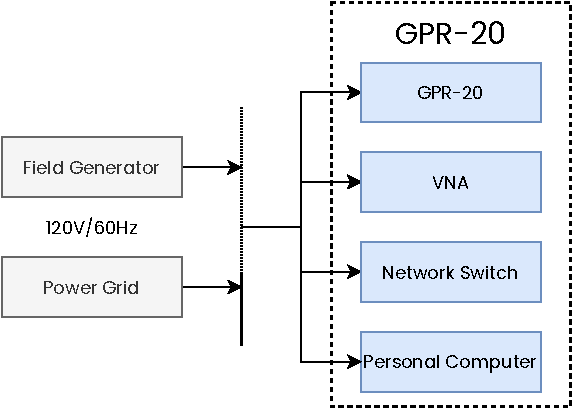
\includegraphics[width=0.7\textwidth]{images/power/GPR20_power_general.pdf}
    \caption{General overview of the GPR-20 power supply systems.}
    \label{fig:power_suplly_global}
\end{figure}

The VNA, network switch and personal computer use power adapters that provide their required electrical energy thus no further analysis can be provided. Nevertheless, the GPR-20 robot has a power-deliver architecture that was designed to satisfy the electrical requirements from its electronic components. The used electronic components of the GPR-20 robot require different voltage levels and electrical characteristics in order to operate safely and appropriately. A diagram of the GPR-20 power system and its distribution is presented in figure \ref{fig:gpr20_power}. Table \ref{tab:gpr20_power_components} expands the information on the power supply system  components. 

\begin{figure}[h]
    \centering
    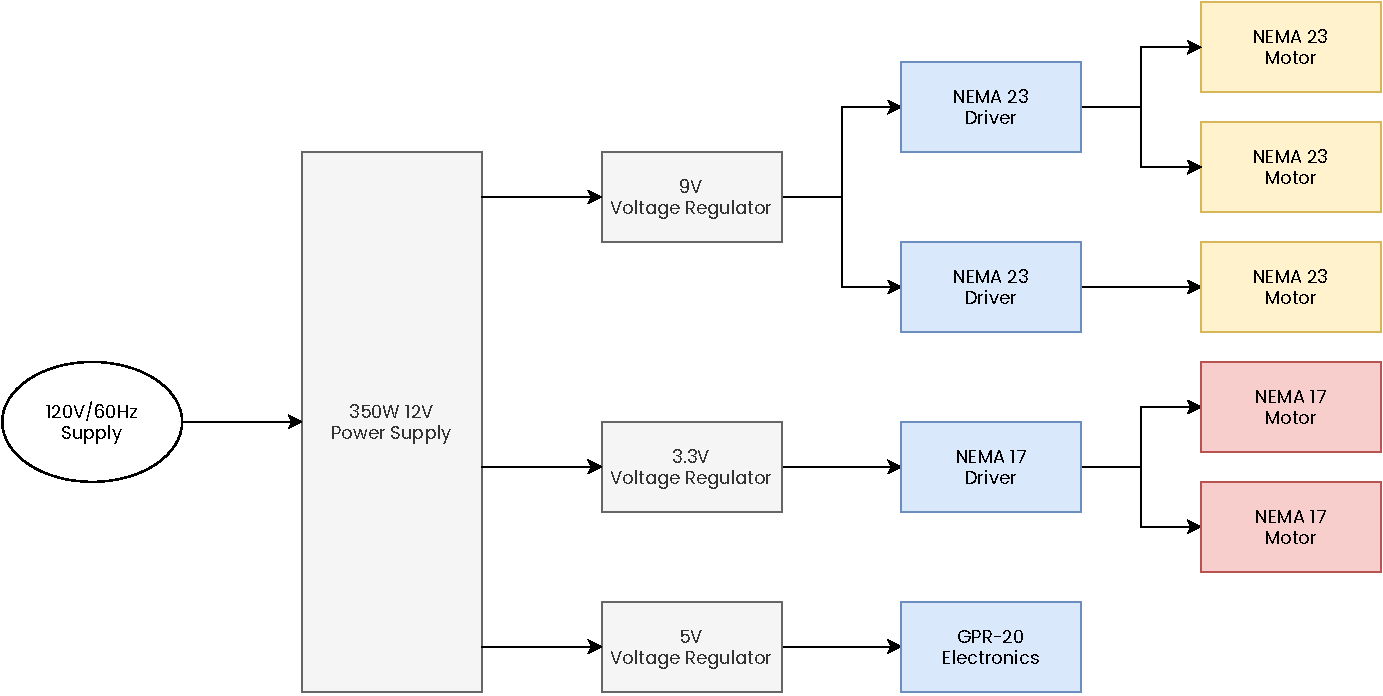
\includegraphics[width=\textwidth]{images/power/GPR20_robot_power.pdf}
    \caption{Power supply diagram of the GPR-20 robot.}
    \label{fig:gpr20_power}
\end{figure}

\begin{singlespace}
    \begin{xltabular}{\textwidth}{|X|l|l|l|}
    
        \hline \textbf{Component} & \textbf{Manufacturer} & \textbf{Reference} & \textbf{Datasheet} \\ \hline
        \endhead
        
        \hline \textbf{Component} & \textbf{Manufacturer} & \textbf{Reference} & \textbf{Datasheet} \\ \hline
        \endfirsthead
        
        \hline \multicolumn{4}{|c|}{\textit{Continues in next page.}} \\ \hline
        \endfoot
        
        \caption{Power supply components with their specific information.} \label{tab:gpr20_power_components}
        \endlastfoot
        
        350W 12V Power Supply & Mean Well & LRS-350-12 & \href{https://www.meanwell.com/productPdf.aspx?i=459\#1}{Link} \\ \hline
        9V Voltage Regulator & Pololu & 4094 & \href{https://www.pololu.com/product/4094}{Link} \\ \hline
        3.3V Voltage Regulator & Pololu & 4090 & \href{https://www.pololu.com/product/4090}{Link} \\ \hline
        5V Voltage Regulator & Pololu & 2850 & \href{https://www.pololu.com/product/2850}{Link} \\ \hline
        NEMA 23 Driver & Pololu & 2133 & \href{https://www.pololu.com/product/2133}{Link} \\ \hline
        NEMA 17 Driver & Pololu & 2134 & \href{https://www.pololu.com/product/2134}{Link} \\ \hline
        NEMA 23 Motor & Pololu & 1477 & \href{https://www.pololu.com/product/1477}{Link} \\ \hline
        NEMA 17 Motor & Pololu & 2267 & \href{https://www.pololu.com/product/2267}{Link} \\ \hline
        
    \end{xltabular}
\end{singlespace}

The main element of the robot power system is the 350W 12V power supply. This element receives a 120V/60Hz AC input and produces a stable 12V DC output. A 12V output was selected in order to use step-down voltage converters only. The power supply can deliver up to 350W which are mostly consumed by the motors. Table \ref{tab:motor_current} presents the used motors and their current consumption. A total of 76.44W are drawn from the power supply for powering the motors. An additional overhead must be added to account for the energy loses on both the voltage converters and motor drivers. According to the voltage regulators' documentation, their efficiency is close to 95\% based on the current draw and input voltage of each device. No information is available for the stepper motor drivers, thus a 90\% efficiency value is used as experimental results indicate similar values. A total power consumption of 89.4W (25.54\%) are used in powering the motors when the efficiency of the converters and drivers is considered in the calculation. 

\begin{table}[h]
    \centering
    \begin{tabular}{|l|l|r|r|}
        \hline \textbf{Motor} & \textbf{Current Consumption} & \textbf{Voltage} & \textbf{Power Draw} \\ \hline
        X-Axis motor (NEMA 23) & 1.0A per coil (two coil) & 9.0V & 18.00W \\ \hline
        Y-Axis left motor (NEMA 23) & 1.0A per coil (two coil) & 9.0V & 18.00W \\ \hline
        Y-Axis right motor (NEMA 23) & 1.0A per coil (two coil) & 9.0V & 18.00W \\ \hline
        Right antenna motor (NEMA 17) & 1.7A per coil (two coil) & 3.3V & 11.22W \\ \hline
        Left antenna motor (NEMA 17) & 1.7A per coil (two coil) & 3.3V & 11.22W \\ \hline \hline
        \multicolumn{3}{|r|}{Total power consumption} & 76.44W \\ \hline
    \end{tabular}
    \caption{GPR-20 motors power consumption.}
    \label{tab:motor_current}
\end{table}

The electronic components are powered through the 5V voltage regulator. Powered components include the on-board computer, touchscreen, IR sensor, ADC and endstop sensors. The main power consumer is the on-board computer that draws 15W from the power supply. The touchscreen draws 3W from the power supply while the remaining components are rated at 2.5W. In this sense, a total of 20.5W of power are required to energize the electronic components of the robot. By accounting for the 95\% efficiency of the voltage converter, a total of 21.57W (6.17\%) are drawn to power the robot electronics. Nevertheless, it must be noted that these values could potentially change by using a different on-board computer. An average upgrade computer for the robot might increase power consumption from 15W to 60W. This would imply a 68.95W (19.7\%) power draw from the power supply.

By factoring the power draw of the motors and the electronics, a total of 110.97W are drawn from the robot power supply. The 110.97W are equivalent to a 31.71\% load of the power supply which in turn ensures a safe operation. A safe operation is defined as a condition in which the power supply has no risk of overheating or overloading. On the other hand, a low load value allows to implement changes without increasing the power supply rating. This is relevant as the robot might sustain changes of its on-board computer and electronics.

\clearpage
\section{Electronics}
This section presents how the electronic systems of the robot are connected and arranged in order to ensure a safe operation. This section will be divided into subsections to explain each of the robot features in the context of its electronics. Finally, a subsection will be dedicated to the Printed Circuit Board (PCB) that was designed for the GPR-20 robot.

\subsection{Motors}
The GPR-20 robot has three degrees-of-freedom: two linear axes and a single rotational axis. The axes movement is accomplished by using stepper motors. Two models of stepper motors are used depending on the axis load: NEMA23 and NEMA17. The motors specifications are presented in table \ref{tab:motor_specs}. Two NEMA23 motors are required for the robot to move the X-Axis and GPR support over the Y axis. A single NEMA23 motor is used to move the GPR support linearly along the X-Axis. Finally, two NEMA17 motors are used to provide the Z-rotation of the motor, that is accomplished by moving the two antennae.

\begin{table}[h]
    \centering
    \begin{tabular}{|l|l|l|}
        \hline \textbf{Specification} & \textbf{NEMA23} & \textbf{NEMA17} \\ \hline
        Holding torque & 14 kg-cm & 3.7kg-cm \\ \hline
        Current rating & 1A per coil & 1.68A per coil \\ \hline
        Voltage rating & 8.6V & 2.8V \\ \hline
        Shaft diameter & 6.35mm "D" & 5mm "D" \\ \hline
        Datasheet & \href{https://www.pololu.com/product/1477}{Link} & \href{https://www.pololu.com/product/2267}{Link} \\ \hline
    \end{tabular}
    \caption{Stepper motor specifications.}
    \label{tab:motor_specs}
\end{table}

 As its name suggest, stepper motors do not move in a continuous rotation but in steps, which corresponds to a 1.8 degree rotation. Each of the stepper motors needs to be controlled by a driver in order to execute the intended movement. Besides from driving the motor coils, motor drivers also provide safety mechanism to avoid permanent damage to the motors. Safety mechanism include reverse-polarity protection and current-limiting for the motor coils. Motors also need to be driven at specific voltage levels in order to ensure that steps will execute as expected. These voltage levels are provided by voltage regulators. However, it must be noted that motors can operate at voltage levels close to their nominal value. This situation is present in the robot motors as no fixed voltage regulator is commercially available for the selected NEMA23 and NEMA17 motors. 

\begin{figure}[h]
    \centering
    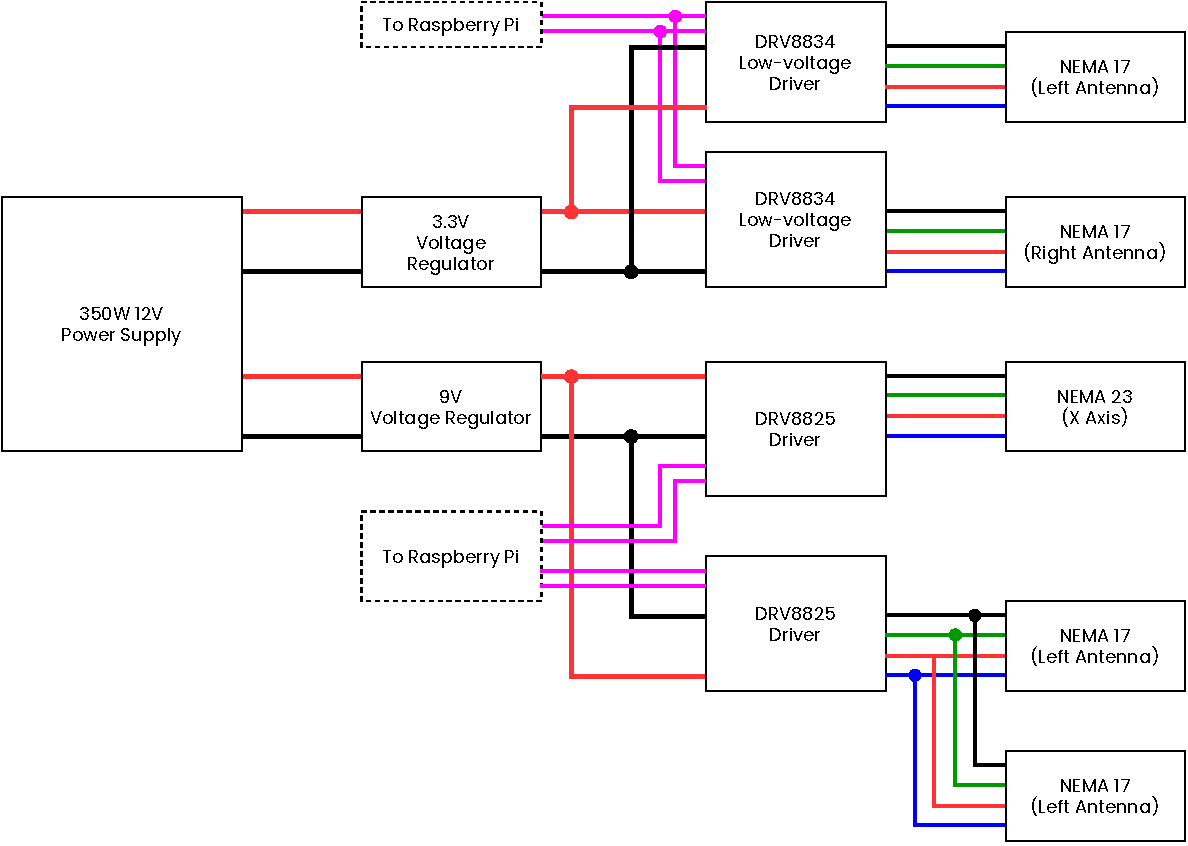
\includegraphics[width=\textwidth]{images/electronics/motor/GPR20_motor_conn.pdf}
    \caption{Motor connection diagram for the GPR-20 robot.}
    \label{fig:motor_conn}
\end{figure}

Figure \ref{fig:motor_conn} presents the motor connection diagram for the GPR-20 robot. Expanded information on figure \ref{fig:motor_conn} components is presented in table \ref{tab:gpr20_power_components}. Raspberry Pi connections are detailed in table \ref{tab:motor_conn_pin}. This table presents each component from diagram \ref{fig:motor_conn}

The motors are connected to their corresponding drivers using four cables. Cables are arranged in pairs, with each pair corresponding to a single coil. Five motors are used in the robot: three for the linear X and Y axes and two for the rotational Z axis. The Y axis motors are connected in parallel to a single driver in order to execute the steps simultaneously. A similar approach is used for the antennae motors in which two drivers are controlled by the same digital signals. Drivers are configured to provide the nominal current for the motors by engaging the built-in current limiters. Drivers are powered with two different voltage levels: 3.3V and 9V. Linear NEMA23 motors use 9V while rotational NEMA23 motors use 3.3V.

\begin{singlespace}
    \begin{xltabular}{\textwidth}{|X|l|X|l|}
        
        \hline \textbf{Upstream Component} & \textbf{Pin} & \textbf{Downstream Component} & \textbf{Pin} \\ \hline
        \endhead
        
        \hline \textbf{Upstream Component} & \textbf{Pin} & \textbf{Downstream Component} & \textbf{Pin} \\ \hline
        \endfirsthead
        
        \hline \multicolumn{4}{|c|}{\textit{Continues in next page.}} \\ \hline
        \endfoot
        
        \caption{Pin connections details. Raspberry Pi 4 GPIO numbering corresponds to \textit{BOARD} numbering.} \label{tab:motor_conn_pin}
        \endlastfoot
        
        350W 12V Power Supply & V+ & 3.3V Voltage Regulator &  V\textsubscript{in} \\ \hline
        350W 12V Power Supply & V- & 3.3V Voltage Regulator & GND \\ \hline
        350W 12V Power Supply & V+ & 9.0V Voltage Regulator &  V\textsubscript{in} \\ \hline
        350W 12V Power Supply & V- & 9.0V Voltage Regulator & GND \\ \hline
        3.3V Voltage Regulator & V\textsubscript{out} & DRV8834 & !SLEEP \\ \hline
        3.3V Voltage Regulator & V\textsubscript{out} & DRV8834 & GND \\ \hline
        9.0V Voltage Regulator & V\textsubscript{out} & DRV8825 & !RESET, !SLEEP \\ \hline
        9.0V Voltage Regulator & V\textsubscript{out} & DRV8825 & GND \\ \hline
        DRV8834 & B2 & NEMA 17 & A (Black) \\ \hline
        DRV8834 & B1 & NEMA 17 & C (Green) \\ \hline
        DRV8834 & A1 & NEMA 17 & B (Red) \\ \hline
        DRV8834 & A2 & NEMA 17 & D (Blue) \\ \hline
        Raspberry Pi 4 & 11 & DRV8834 & DIR \\ \hline
        Raspberry Pi 4 & 12 & DRV8834 & STEP \\ \hline
        DRV8825 & B2 & NEMA 23 & A (Black) \\ \hline
        DRV8825 & B1 & NEMA 23 & C (Green) \\ \hline
        DRV8825 & A1 & NEMA 23 & B (Red) \\ \hline
        DRV8825 & A2 & NEMA 23 & D (Blue) \\ \hline
        Raspberry Pi 4 & 13 & DRV8825 (X-Axis) & DIR \\ \hline
        Raspberry Pi 4 & 15 & DRV8825 (X-Axis) & STEP \\ \hline
        Raspberry Pi 4 & 37 & DRV8825 (Y-Axis) & DIR \\ \hline
        Raspberry Pi 4 & 38 & DRV8825 (Y-Axis) & STEP \\ \hline
    \end{xltabular}
\end{singlespace}

Digital signals are used to control the amount of steps that are required to be executed by the motor. Motor drivers are controlled by the same protocol despite being two different models. The protocol uses two digital signals that control the stepping action and the movement direction. Stepping action is executed on the rising edge of the signal. When executing multiple steps, the stepping signal will be similar to a square wave. Direction pin depends on the logic level of the signal thus no wave-like behavior is expected. Digital signals are driven from the Raspberry Pi 4 on-board computer.

\subsection{Sensors}
Height and endstop sensors are used to acquire data different of the GPR. This data is crucial for operating the robot and improving the GPR data quality. Height data is used to provide a GPR measurement 
with a value of the antennae height. The antennae height serves as a reference that is used in the GPR data processing. Endstop sensors are used to provide the reference point of the linear axes of the robot. Despite not being the zero (0) coordinate for the axes, the reference point provides a consistent value from which coordinates are referred. The height and endstop sensor data is fed to the on-board computer using digital signals. Specifications for the endstop sensor and height sensor are provided in table \ref{tab:sensors_specs}.

\begin{table}[h]
    \centering
    \begin{tabular}{|l|l|l|}
        \hline \textbf{Specification} & \textbf{Height Sensor} & \textbf{Endstop Sensor} \\ \hline
        Reference & GP2Y0A21YK0F & SEN0138-R \\ \hline
        Operating voltage & 4.5V to 5.5V & 5.0V \\ \hline
        Sensor type & Distance measurement & Endstop sensor \\ \hline
        Manufacturer & SHARP & DFRobot \\ \hline
        Datasheet & \href{https://www.pololu.com/file/0J85/gp2y0a21yk0f.pdf}{Link} & \href{https://www.dfrobot.com/product-763.html}{Link} \\ \hline
    \end{tabular}
    \caption{Specifications for the height sensor and endstop sensor.}
    \label{tab:sensors_specs}
\end{table}

Endstop sensors provide a three-port interface in order to use them. The device uses a input voltage, ground connection and a logical output. Both the input voltage and the ground connection are provided by the voltage converter. The logical output is connected to the on-board computer to be used by the control software. The logical output is continuously driven by an integrated pull-up resistor unless the switch is pressed. A pressed sensor will drive the logical output low.

The height sensor uses infrared light to measure distances from ten (10) centimeters up to eighty (80) centimeters. The sensor requires an input voltage and ground connections to operate, which are in turn provided by the voltage converter. The output of the sensor is analog thus an analog/digital converter (ADC) must be integrated for the on-board computer to use the data. The ADC receives the input analog data and then convert it to a digital value that is transmitted using the SPI protocol. The digital distance value can take up to 1024 different values (10-bit resolution). The ADC has the same voltage reference value as the height sensor in order to avoid measurement errors.

\begin{figure}[h]
    \centering
    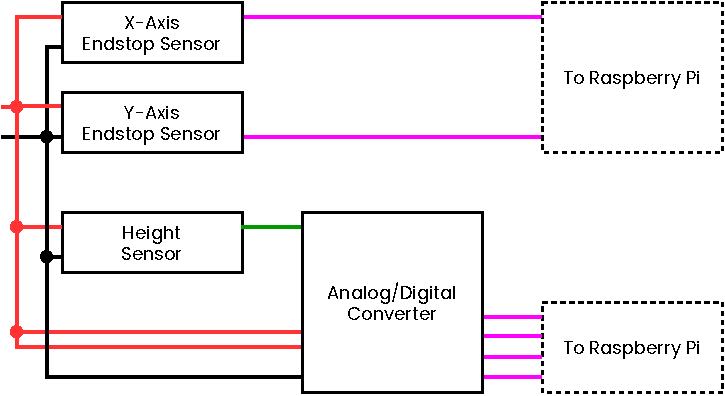
\includegraphics[width=0.7\textwidth]{images/electronics/sensors/GPR20_sensors_conn.pdf}
    \caption{Connection diagram for the GPR-20 sensors.}
    \label{fig:sensors_conn}
\end{figure}

\begin{singlespace}
    \begin{xltabular}{\textwidth}{|X|l|X|l|}
        \hline \textbf{Upstream Component} & \textbf{Pin} & \textbf{Downstream Component} & \textbf{Pin} \\ \hline
        \endhead
        
        \hline \textbf{Upstream Component} & \textbf{Pin} & \textbf{Downstream Component} & \textbf{Pin} \\ \hline
        \endfirsthead
        
        \hline \multicolumn{4}{|c|}{\textit{Continues in next page.}} \\ \hline
        \endfoot
        
        \caption{Sensors connections details. Raspberry Pi 4 GPIO numbering corresponds to \textit{BOARD} numbering.} \label{tab:sensors_conn}
        \endlastfoot
        
        5V Voltage Regulator & V\textsubscript{out} & Endstop Sensor & VCC \\ \hline
        5V Voltage Regulator & V\textsubscript{out} & Endstop Sensor & GND \\ \hline
        Endstop Sensor (X-Axis) & OUT & Raspberry Pi 4 & 16 \\ \hline
        Endstop Sensor (Y-Axis) & OUT & Raspberry Pi 4 & 40 \\ \hline
        5V Voltage Regulator & V\textsubscript{out} & Height Sensor & V\textsubscript{CC} \\ \hline
        5V Voltage Regulator & GND & Height Sensor & GND \\ \hline
        Height Sensor & V\textsubscript{O} & Analog/Digital Converter & CH0 \\ \hline
        5V Voltage Regulator & V\textsubscript{out} & Analog/Digital Converter & V\textsubscript{DD}, V\textsubscript{REF} \\ \hline
        5V Voltage Regulator & GND & Analog/Digital Converter & DGND, AGND \\ \hline
        Raspberry Pi 4 & 23 (SCLK) & Height Sensor & SCLK \\ \hline
        Raspberry Pi 4 & 24 (CE0) & Height Sensor & !CS \\ \hline
        Raspberry Pi 4 & 19 (MOSI) & Height Sensor & MISO \\ \hline
        Height Sensor & MISO & Raspberry Pi 4 & 21 \\ \hline
    \end{xltabular}
\end{singlespace}

\clearpage

Figure \ref{fig:sensors_conn} presents the connection diagram for the GPR-20 robot sensors. Table \ref{tab:sensors_conn} presents the connection of components from figure \ref{fig:sensors_conn}. Datasheets and expanded information on the components are presented in table \ref{tab:sensors_specs}. Three different device types are included in the diagram: endstop sensors, height sensor and ADC. The robot has two (2) endstop sensors that are included in each linear axis. The endstop sensors are powered from the 5V voltage converter. The endstop sensors output is fed directly into the Raspberry Pi on-board computer. A single height sensor is used in the robot. The height sensor is also powered by the 5V voltage converter. The sensor output is then fed into the ADC for its conversion into a digital 10-bit value. The 5V voltage supply is used in the ADC for two purposes: to power the device, and to provide a reference voltage for the conversions. The output converted value is transmitted to the on-board computer using the SPI protocol. The SPI protocol uses four (4) digital signals to transmit data: a clock, transmitter-to-receiver data, receiver-to-transmitter data and chip select. The Raspberry Pi will act as the transmitter and the ADC will act as the receiver in the GPR-20 robot.

\subsection{Others}
The GPR-20 makes use of different devices to provide all of its functionalities. Devices such as the Vector Network Analyzer (VNA), the touchscreen and personal computer use standard communication mechanisms to interact between them. This subsection will discuss how these connections are achieved. Networking between VNA, personal computer and the GPR-20 robot is achieved through a Local Area Network (LAN) governed by a switch. The connection between devices is done using Ethernet cables as wireless networking might interfere with the GPR operation. Internet connection will depend on the service availability on location. Figure \ref{fig:gpr20_network} presents the network configuration of the GPR-20 devices. 

\begin{figure}[h]
    \centering
    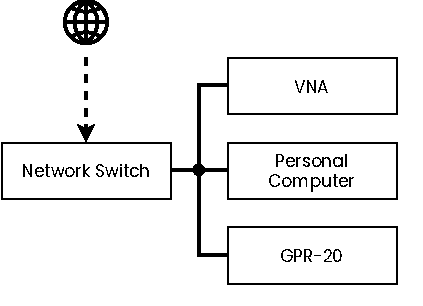
\includegraphics[width=0.6\textwidth]{images/electronics/others/GPR20_networking.pdf}
    \caption{GPR-20 network configuration.}
    \label{fig:gpr20_network}
\end{figure}

The GPR-20 touchscreen (\href{https://www.adafruit.com/product/2406}{datasheet}) is driven by an USB and HDMI connection with the on-board computer. The USB communication provides the touch information and powers supply for the screen whilst the HDMI carries the display data. The USB connection is supposed to be provided by the on-board computer although this is not implemented in the GPR-20 robot. The Raspberry Pi is powered from a 5V voltage converter although not directly. The 5V voltage converter is used to drive an USB cable that powers the on-board computer. This causes the voltage to drop from 5V which leads the Raspberry Pi to be in an undervoltage configuration. If the touchscreen is driven from the Raspberry Pi, the former will not receive the appropriate input voltage and will cease to work. To avoid a failure from the touchscreen it is driven directly from the 5V voltage regulator. It must be noted that failing to power the touchscreen from the Raspberry Pi will prevent the touch operation from working. Software solutions and upgrades will be considered to restore the intended connection for the Raspberry Pi.


\subsection{PCB}
A Printed Circuit Board was designed and manufactured in order to provide the GPR-20 robot with reliable electronics. The PCB was designed using the open-source CAD program \href{https://www.kicad.org/}{KiCAD}. The design files for the PCB are stored in their corresponding repository (\href{https://github.com/gdh-uniandes/gpr20_pcb}{link}). Motor control and sensors circuits and power supply systems are incorporated into the robot's PCB. The PCB has the appropriate routing to power different devices and to provide the control/data ports that are required to be connected to the on-board computer. Figure \ref{fig:pcb_diagram} presents the PCB for the GPR-20 robot. Figure \ref{fig:pcb_components} presents the PCB with the components footprint highlighted. Table \ref{tab:pcb_components} presents a breakout of further information on the board components.

\begin{figure}[h]
    \centering
    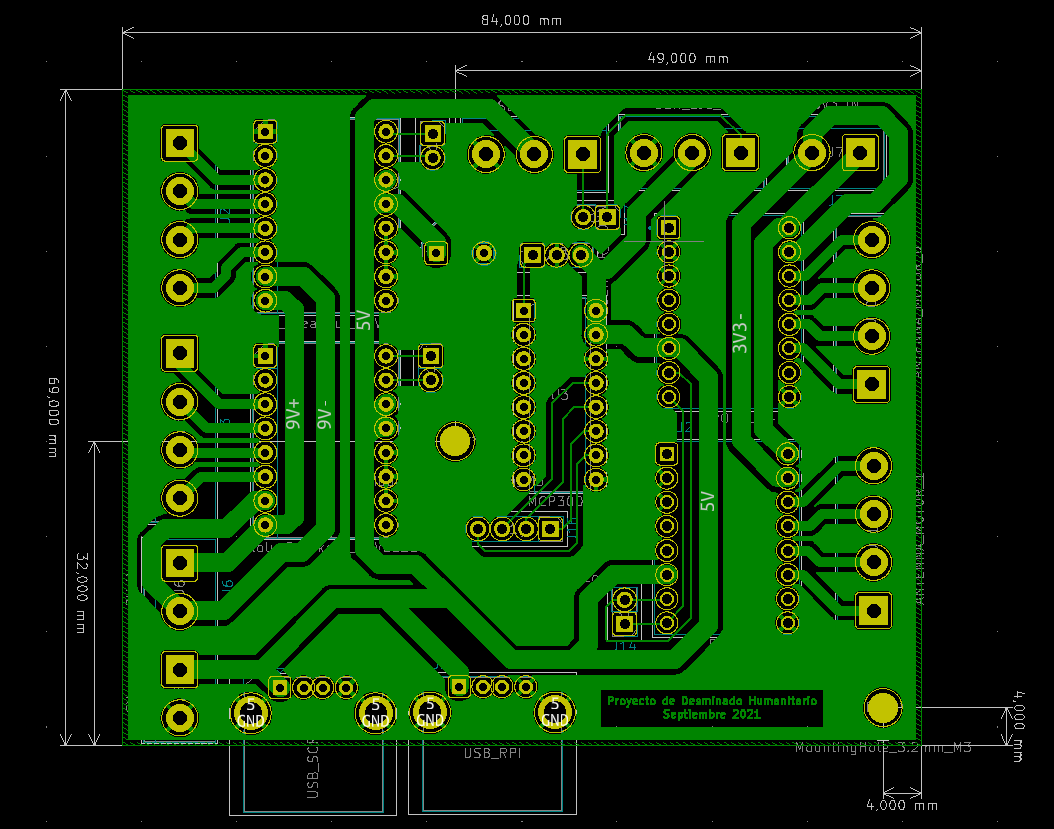
\includegraphics[width=0.7\textwidth]{images/electronics/pcb/dimensiones.png}
    \caption{PCB design for the GPR-20 robot.}
    \label{fig:pcb_diagram}
\end{figure}

\begin{singlespace}
    
    \begin{xltabular}{\textwidth}{|X|l|X|}
        
        \hline \textbf{Name} & \textbf{ID} & \textbf{Component} \\ \hline
        \endhead
        
        \hline \textbf{Name} & \textbf{ID} & \textbf{Component} \\ \hline
        \endfirsthead
        
        \hline \multicolumn{3}{|c|}{\textit{Continues in next page.}} \\ \hline
        \endfoot
        
        \caption{PCB components breakout.} \label{tab:pcb_components}
        \endlastfoot
        
        DRV8825 & A1, A2 & $2\times8$ Pin Header (0.1") \\ \hline
        $1000\mu$F & C1 & $1000\mu$F Capacitor \\ \hline
        USB\_RPI & J1 & A-Type USB connector \\ \hline
        X\_AXIS\_MOTOR & J2 & 4-Pin Terminal Block \\ \hline
        Y\_AXIS\_MOTOR & J3 & 4-Pin Terminal Block \\ \hline
        USB\_SCREEN & J4 & A-Type USB connector \\ \hline
        5V\_IN & J5 & 2-Pin Terminal Block \\ \hline
        9V\_IN & J6 & 2-Pin Terminal Block \\ \hline
        3V3\_IN & J7 & 2-Pin Terminal Block \\ \hline
        SEN\_EJE\_X & J8 & 3-Pin Terminal Block \\ \hline
        SEN\_EJE\_Y & J9 & 3-Pin Terminal Block \\ \hline
        ANTENNA\_MOTOR\_0 & J10 & 4-Pin Terminal Block \\ \hline
        ANTENNA\_MOTOR\_1 & J11 & 4-Pin Terminal Block \\ \hline
        X-Axis Input & J12 & 2-Pin Header (0.1") \\ \hline
        Y-Axis Input & J13 & 2-Pin Header (0.1") \\ \hline
        Antennae Input & J14 & 2-Pin Header (0.1") \\ \hline
        Height Sensor Input & J15 & 3-Pin Header (0.1") \\ \hline
        SPI Output & J16 & 4-Pin Header (0.1") \\ \hline
        Endstop Sensor Output & J17 & 2-Pin Header (0.1") \\ \hline
        DRV8834 & U1, U2 & $2\times8$ Pin Header (0.1") \\ \hline
        MCP3008 & U3 & DIP-16 IC Bed \\ \hline
    \end{xltabular}
\end{singlespace}

Motor control was found to be affected by noise and grounding issues during the robot development. Failing to provide an appropriate grounding was found to be the cause of undesired movement on the motors. Motor vibrations were found to be related to noise and caused vibrations which in turn affected the mechanical structure. These problems were mitigated by mounting the motor electronics on the PCB. The PCB was designed to include the appropriate grounding and to reduce the noise on the routing. 

\begin{figure}[h]
    \centering
    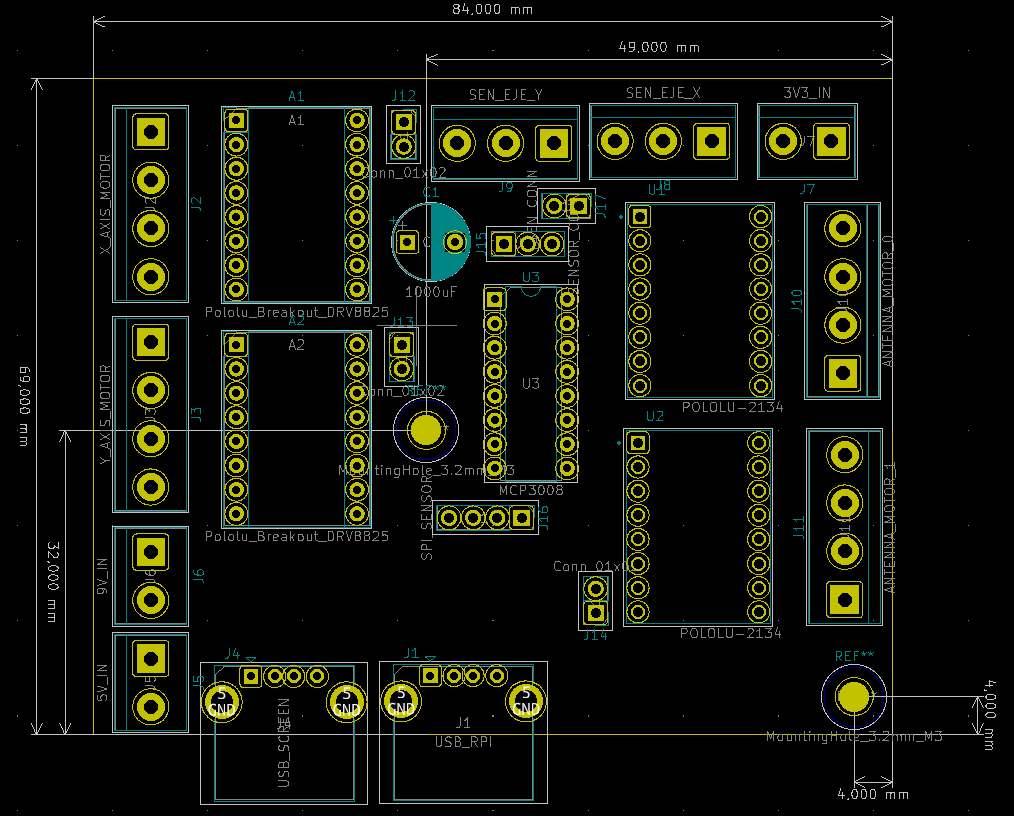
\includegraphics[width=0.7\textwidth]{images/electronics/pcb/GPR20_PCB_components.png}
    \caption{PCB with the components highlighted.}
    \label{fig:pcb_components}
\end{figure}

The PCB was used to provide the power supply of different devices. Endstop sensors and height sensors were powered from the 5V voltage level provided by the corresponding voltage regulator. A similar approach was used for the Raspberry Pi 4 and touchscreen devices. The difference was that the on-board computer and the input mechanisms used a USB connector for powering purposes. 

Motors also were powered by the PCB routing since their drivers were mounted on the board. Inputs for the motor's power supply are provided in the PCB and routing considered the amount of current used by them. Each of the motors are connected to the PCB via terminal blocks. Finally, mounting holes were implemented in the PCB to securely mount the board.

\end{document}
